\chapter{使用真核生物 RNA-Seq 数据通过最大似然辨识基因的剪切异构体是一个 NP 难问题}
\label{chap-rna-seq-nphard}

\section{问题描述}
在真核生物 RNA-Seq 数据处理过程当中, 重要的一步是通过 RNA-Seq 数据识基因的不同的剪切异构体。 
由于在真核生物的转录过程当中会有选择性剪切的现象发生, 一个基因可能转录出多个剪切异构体。 
在这种情况下, 我们需要通过 RNA-Seq 数据辨识出基因的不同的剪切异构体。 

在 RNA-Seq 实验中得到的读段数据在比对到参考基因组序列上如图 \ref{nphard.ex1.aligned.data} 所示. 
对于 RNA-Seq 数据, 
我们可以通过序列拼装工具 (例如 Trinity \cite{grabherr2011full} 等) 进行拼装。 
得到每一个基因的外显子的序列以及这些外显子之间是如何连接在一起的关系, 
从而得到每一个基因的剪切图 \cite{Heber01072002}。 
在有基因的参考序列以及基因注释的情况下, 也可以直接通过基因注释获得每一个基因的剪切图。 
对于图 \ref{nphard.ex1.aligned.data} 中所示的基因和 RNA-Seq 数据, 
通过 Trinity 拼装获得的剪切图如图 \ref{nphard.ex1.splicing.graph} 所示。 

\begin{figure}[!t]
\centering
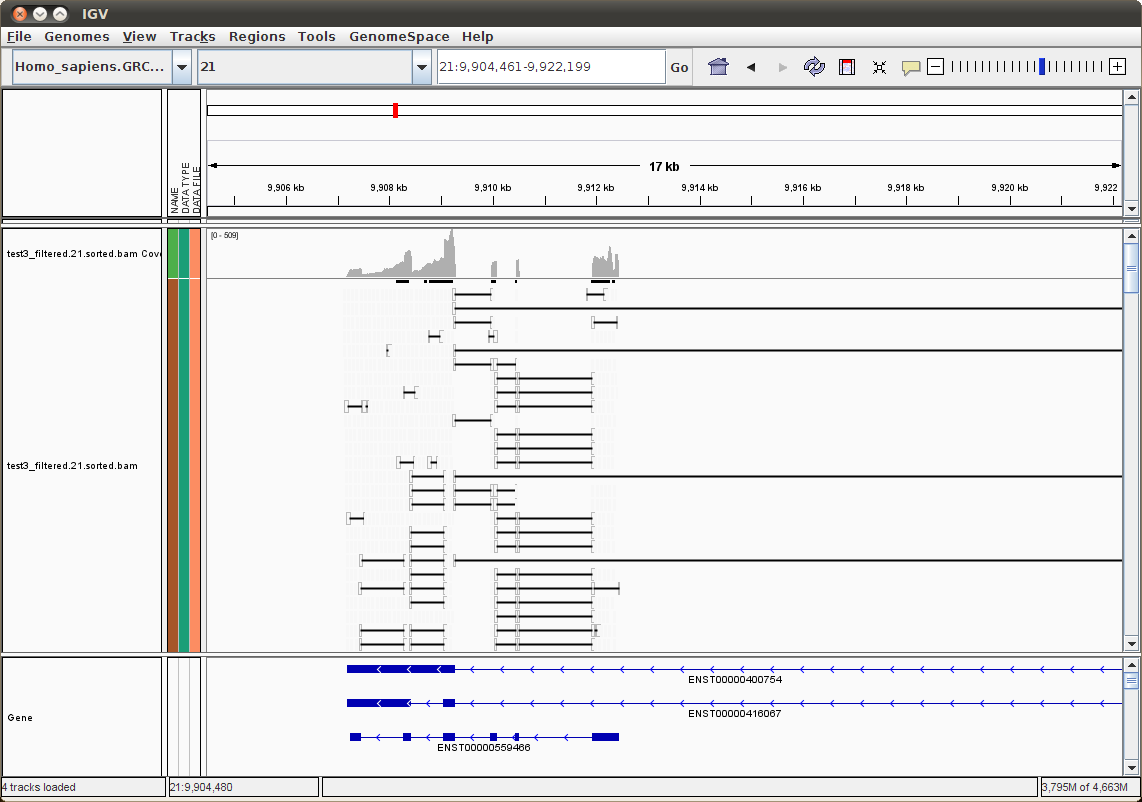
\includegraphics[width=\textwidth]{figures/nphard/comp1.png}
\caption[一个基因的比对到基因组参考序列上的 RNA-Seq 数据]
{一个基因的比对到基因组参考序列上的 RNA-Seq 数据: 
根据每一个读段比对到基因组参考序列上的位置可以确定其所对应的剪切异构体。}
\label{nphard.ex1.aligned.data}
\end{figure}

\begin{figure}[!t]
\centering
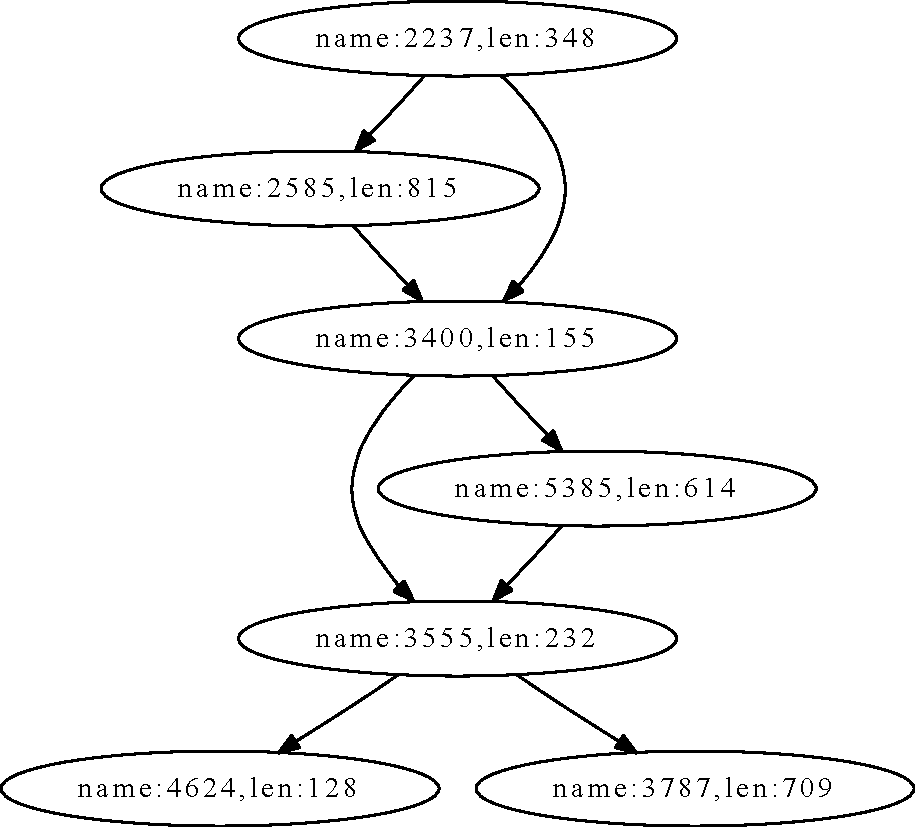
\includegraphics[width=\textwidth]{figures/nphard/comp1.pdf}
\caption[图 \ref{nphard.ex1.aligned.data} 中所示的基因和 
RNA-Seq 数据通过 Trinity \cite{grabherr2011full} 拼装得到的剪切图]
{图 \ref{nphard.ex1.aligned.data} 中所示的基因和 
RNA-Seq 数据通过 Trinity \cite{grabherr2011full} 拼装得到的剪切图: 
该基因的一个剪切异构体是这个图中的一条路径。}
\label{nphard.ex1.splicing.graph}
\end{figure}

\subsection{模型}
\label{nphard-model}

为了能够通过 RNA-Seq 数据辨识每个基因的剪切异构体, 
我们在这里介绍一个 Poisson 模型用来描述 RNA-Seq 数据 \cite{Jiang15042009}。 
该模型与 \ref{rna-seq-general-model} 中所介绍的多项式模型在数学上是等价的 
\cite{2011arXiv1104.3889P}。 
在这里采用 RNA-Seq 数据的 Poisson 模型是为了简化问题的描述。 

另外, 为了叙述的方便, 我们在这里纸考虑辨识一个基因的剪切异构体。 

对于真核生物中的一个基因, 根据剪切图的定义, 
我们将其表示为一个有向无环图 $G=(V,E)$, 其中 $G$ 中的一个节点代表一个外显子, 
节点 $v_i$ 到 $v_j$ 有一条边当且仅当在这个基因当中有一个剪切异构体同时包含 
$v_i$ 和 $v_j$ 所代表的外显子, 
同时在这个剪切异构体中 $v_i$ 和 $v_j$ 所代表的外显子是相邻的, 
并且 $v_i$ 代表的外显子在 $v_j$ 代表的外显子的 5' 上端。 

该基因的一个剪切异构体是图 $G$ 中的一个路径 $v_1 \to v_2 \to \ldots \to v_k$, 
其中 $v_i$, $i=1,2,\ldots,k$ 是构成该剪切异构体的外显子。 
我们用 $I$ 表示这个基因的剪切异构体构成的集合, $\lambda_i \geq 0$, 
$i \in I$ 是剪切异构体 $i$ 的表达量。 

在这里, 我们假设所有的 RNA-Seq 数据均是单端读段, 且长度均为 $k$。 
(对于长度不均的读段或者双端测序的读段我们可以采用与这里类似的方法进行处理, 
此处不再赘述, 感兴趣的读者可以参看 \onlinecite{cufflinks.2010}。) 
一个读段对应到剪切图中时, 该读段对应到原转录本上的每一个外显子在剪切图中所对应的节点, 
同时在读段经过多个外显子时该读段也会经过剪切图中所对应的边。 
为了描述的方便, 我们把每一个读段对应在原转录本上的 5' 端的位置称之为该读段的起始位置, 
对应在原转录本上的 3' 端的位置称之为该读段的终止位置。 

我们假设每一个读段可以在该基因中的位置是已知的并且是唯一的 
(对于基因序列的分析表明这样一个假设是合理的 \cite{peng2011t})。 

同时, 我们把该基因在 RNA-Seq 实验中所有对应的读段构成的集合记为 $R$。 

在用来描述 RNA-Seq 数据的 Poisson 模型中, 
我们假设对于基因中的每一个位置 $p$, 
在这个位置起始的读段的个数满足参数为 
\begin{equation}
\label{rna-seq-data-position-lambda}
\lambda_p = \sum_{\text{剪切异构体 $i \in I$ 经过位置 $p$}} a_{pi} \lambda_i
\end{equation}
的 Poisson 分布。 (此处可以参考图 \ref{nphard.ex1.aligned.data} 进行理解。)
这里 $a_{pi} \geq 0$ 是与目前该位置 $p$ 有关的一个采样率 \cite{2011arXiv1106.3211S}。 
我们假设在给定基因中的一个位置 $p$ 之后, 以及一个剪切异构体 $i \in I$, 
$a_{pi}$ 是已知的。 
对于理想的情况我们认为对于所有的基因中的位置 $p$ 和剪切异构体 $i\in I$, 
我们均有 $a_{pi}=1$。 
通过设定不同的位置和不同的剪切异构体 $i\in I$ 的 $a_{pi}$, 
我们可以对 RNA-Seq 实验中存在的不均匀性进行建模。 
为了方便下面的陈述, 我们记基因中所有可以有读段起始的位置的集合记作 $P$。 
(例如, 对于一个只有一个外显子的基因, 其长度为 $L$, 
$P$ 由该基因上的前 $L-k+1$ 个位置组成。)

同时, 我们假设对于该基因中不同的位置, 
在这些位置起始的读段的个数的分布是独立的。 

根据上面的描述, 我们得出观察到 RNA-Seq 读段的似然函数
\begin{equation}
\label{rna-seq-data-poisson-likelihood}
L(R)= \prod_{p\in P} \frac{{\lambda_p}^{N(p)} e^{-\lambda_p}}{N(p)!}
\end{equation}
其中 $N(p)$ 是在位置 $p\in P$ 所管查到的在该位置起始的读段的数目, 
$\lambda_p$ 如式 \eqref{rna-seq-data-position-lambda} 中所定义。 
注意到 $|R|=\sum_{p\in P}N_p$。

根据式 \eqref{rna-seq-data-poisson-likelihood} 中所给出来的似然函数, 
我们可以通过最大化该似然函数确定该基因的剪切异构体的集合 $I$, 
辨识该基因的剪切异构体 \cite{xing2006expectation}。 
但是由于一个基因可能的剪切异构体的个数是随着该基因中外显子的个数增长按指数规律增长的, 
所以我们可以使用一个带惩罚项的似然函数进行最大化
\begin{align}
\tilde{L}(R) &= e^{-\Phi} L(R) \nonumber \\ 
\label{rna-seq-data-poisson-penalized-likelihood}
&= e^{-\Phi} \prod_{p\in P} \frac{{\lambda_p}^{N(p)} e^{-\lambda_p}}{N(p)!}
\end{align}
其中 $\Phi \geq 0$ 是一个惩罚函数。 

对于这里的乘法函数 $\Phi$ 我们可以选取: 
\begin{itemize}
\item $L_0$ 正则化:
\[
\Phi = \Lambda \sum_{i \in I, \lambda_i \neq 0} 1
\]
其中 $\Lambda \geq 0$ 是一个常数。 

当我们取 
\[
\Lambda = \frac{\log |R|}{2}
\]
此时相当于使用 BIC (Bayesian information criterion) \cite{BIC.Schwarz_1978}。 

\item Lasso \cite{tibshirani1996regression}:
\[
\Phi = \Lambda \sum_{i \in I} |\lambda_i|
\]
其中 $\Lambda \geq 0$ 是一个常数。 

该方法是 NSMAP \cite{nsmap.21575225} 所使用的方法。 

\item $L_q$ ($0<q<1$) 正则化:
\[
\Phi = \Lambda \sum_{i \in I} |\lambda_i|^q
\]
其中 $\Lambda \geq 0$, $0 <q<1$ 为两个常数。 

该方法是 Montebello \cite{Hiller.Montebello} 所使用的方法。 
\end{itemize}

\subsection{M-ISOFORM 判定问题}
为了说明通过真核生物 RNA-Seq 数据估计基因的转录组的问题, 
也即辨识基因的剪切异构体的问题, 我们在这里定义一个判定问题 M-ISOFORM。 

根据 \onlinecite{luenberger2008linear} 我们可以知道, 
当我们使用 $L_0$ 正则化作为式 \eqref{rna-seq-data-poisson-penalized-likelihood} 
中的惩罚函数最大化带惩罚项的似然函数时, 此时等价于
\begin{align}
\max &\ L(R) =  \prod_{p\in P} \frac{{\lambda_p}^{N(p)} e^{-\lambda_p}}{N(p)!} \nonumber \\
\label{rna-seq-data-likelihood-1}
\text{s.t.} &\  \sum_{i \in I, \lambda_i>0} 1 \neq t
\end{align}
其中 $t\geq 0$ 是一个常数。 

%\begin{figure}[!t]
%\centering
%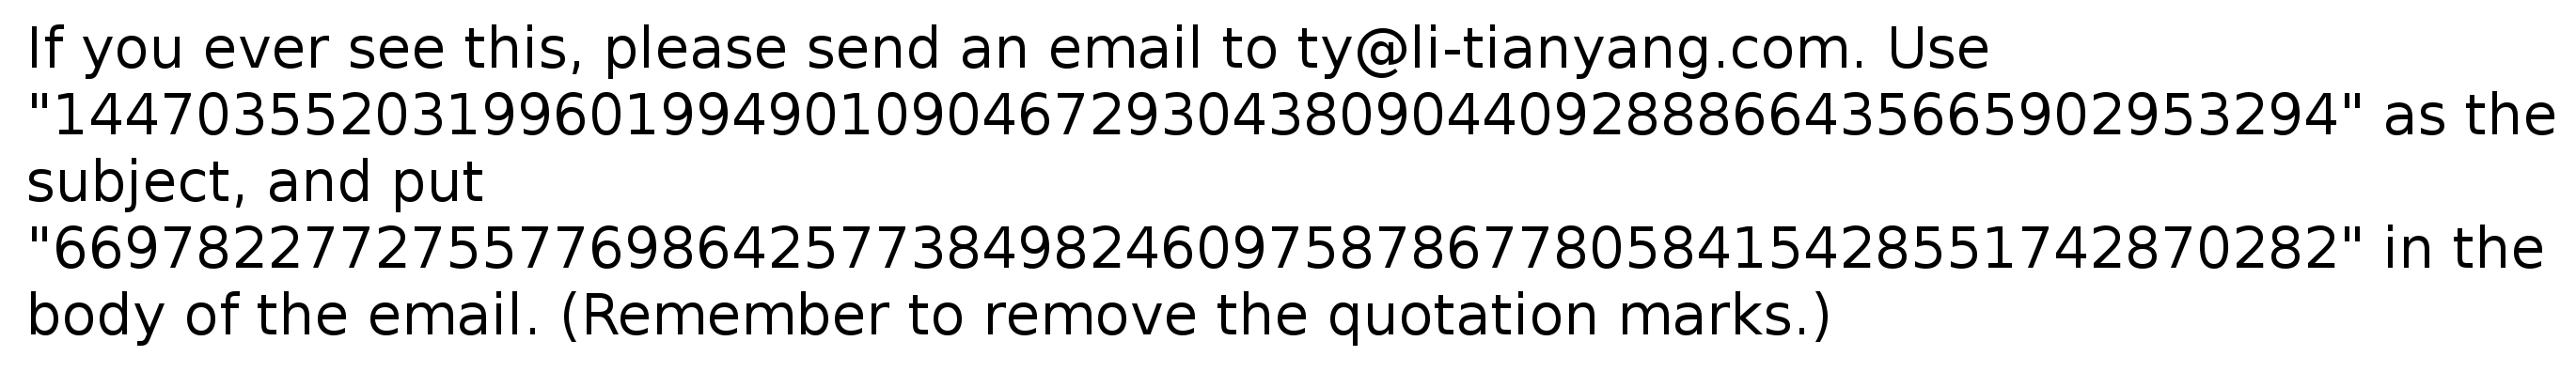
\includegraphics[width=\textwidth]{figures/lol.png}
%\caption*{}
%\end{figure}

同时我们对剪切异构体的集合 $I$ 也有要求: 对于每一个属于 $R$ 的读段 $r$, 
我们均要求至少存在一个剪切异构体 $i \in I$ 使得读段 $r$ 是可以来自剪切异构体 $i$ 的。 
这对于式 \ref{rna-seq-data-likelihood-1} 中的优化问题又增加了一项组合约束。 

给出了这些观察之后, 我们可以将此处通过 RNA-Seq 数据估计转录组中转录本的问题, 
也即基因的剪切异构体的辨识的问题, 转换为一个判定问题:
\begin{center}
\fbox{\parbox{0.8\textwidth}{给定一个阈值, 
能不能找到一个剪切异构体的集合以及这些转录本的表达量使得似然函数的值大于该阈值?}}
\end{center}

下面我们采用前面 \ref{nphard-model} 中所使用的符号来描述判定问题 M-ISOFORM。 

\newtheorem*{misof}{M-ISOFORM}

\begin{center}
\fbox{\parbox{0.8\textwidth}{
\begin{misof}
\hspace*{1mm}

实例: 一个基因的剪切图 $G$, 以及对应到该剪切图中的读段集合 $R$ 
(这里我们保证剪切图 $G$ 中的所有定点所对应的外显子和边所表示的外显子的连接关系均能由 
$R$ 中的读段解释)。 常数 $q \in \mathbb{R}$, $m \in \mathbb{Z}^+$。 

问题: 是否存在该基因的一个剪切异构体的集合 $I$, $|I| \leq m$, 
以及这些转录本的表达量 $\theta_i > 0$
使得式 \eqref{rna-seq-data-poisson-likelihood} 中的似然函数 $L(R) \geq q$, 
并且对每一个读段 $r \in R$ 均存在至少一个该基因的剪切异构体 $i\in I$ 
让读段 $r$ 来自剪切异构体 $i$?
\end{misof}
}}
\end{center}

在实数 RAM 模型 \cite{Preparata:1985:CGI:4333} 下, 
我们下面的定理说明了 M-ISOFORM 是一个 NP 完全问题。 

\begin{center}
\fbox{\parbox{0.8\textwidth}{
\begin{thm}
\label{m-isoform-np-hard}
M-ISOFORM 是一个 NP 完全问题。
\end{thm}
}}
\end{center}

\section{证明}

下面我们给出定理 \ref{m-isoform-np-hard}, 说明 M-ISOFORM 是一个 NP 完全问题。 
定理 \ref{m-isoform-np-hard} 的证明主要受到了 
Tomescu et al. 在 \onlinecite{Tomescu.recomb.seq.2013} 的工作的启发, 
将通过 RNA-Seq 数据辨识基因的剪切异构体的问题看作是一个网络流问题。 
证明中我们采用了一个类似 Vatinlen et al. 在 \onlinecite{Vatinlen20081390} 中所使用的方法, 
将 3-PARTITION \cite{doi:10.1137/0204035, Garey:1990:CIG:574848} 规约到 M-ISOFORM。 

\begin{proof}

首先注意到在实数 RAM 模型 \cite{Preparata:1985:CGI:4333} 下, 
在给定该基因的一个剪切异构体的集合 $I$ 的情况下, 及个转录本的表达量 $\theta_i$, $i\in I$, 
我们可以在多项式时间内验证是否式 \eqref{rna-seq-data-poisson-likelihood} 中的似然函数 $L(R) \geq q$, 
并且对所有的读段 $r\in R$, 
是否存在一个剪切异构体 $i\in I$ 让读段 $r$ 可以来自剪切异构体 $i$。 
所以我们可以看出来 M-ISOFORM $\in$ NP。 

下面处我们介绍判定问题 3-PARTITION \cite{doi:10.1137/0204035, Garey:1990:CIG:574848}, 
并给出一个方法在多项式时间内规将其约到 M-ISOFORM。 

\newtheorem*{tripart}{3-PARTITION}

\begin{center}
\fbox{\parbox{0.8\textwidth}{
\begin{tripart}
\hspace*{1mm}

实例: 一个包含 $3w$ 个元素的集合 $X$, 一个界 $Y \in \mathbb{Z}^+$, 
和一个量 $u(x) \in \mathbb{Z}^+$ 使得对每个 $x \in X$ 
都有 $\frac{Y}{4} < u(x) < \frac{Y}{2}$, 
并且 $\sum_{x \in X} u(x) = w Y$。

问题: $X$ 能否被划分为 $w$ 个不相交的集合 $X_1$, $X_2$, \ldots, $X_w$ 使得, 
对所有的 $1 \leq i \leq w$, $\sum_{x \in X_i} u(x) = Y$ 
(注意到每个 $X_i$ 必须包含恰好 3 个来自 $X$ 的元素)?
\end{tripart}
}}
\end{center}

根据 Garey 和 Johnson 在 \onlinecite{doi:10.1137/0204035} 中以及 
Garey 和 Johnson 在 \onlinecite{Garey:1990:CIG:574848} 的工作, 
我们可以知道 3-PARTITION 是强 NP 完全的, 
即 3-PARTITION 的输入用 unary 表示时 3-PARTITON 仍然是 NP 完全的。 

我们下面将用 unary 输入的一个 3-PARTITION 实例在多项式时间内规约到一个 M-ISOFORM 实例。 

给定一个 unary 输入的 3-PARTITION 的实例, 
我们构造一个基因如图 \ref{tripart-reduce-gene} 所示, 
这里每一个外显子的长度均为 $k-1$ bp ($k\geq 2$ 是一个固定的常数)。 
同时我们构造一个读段的集合 $R$, 
其中共包含 $4wY(k-1)$ 个长度为 $k$ bp 的读段。 
在这里为了方便描述, 我们不妨设 $X=\{1,2,\ldots,3w\}$。 

\begin{figure}[!t]
\centering
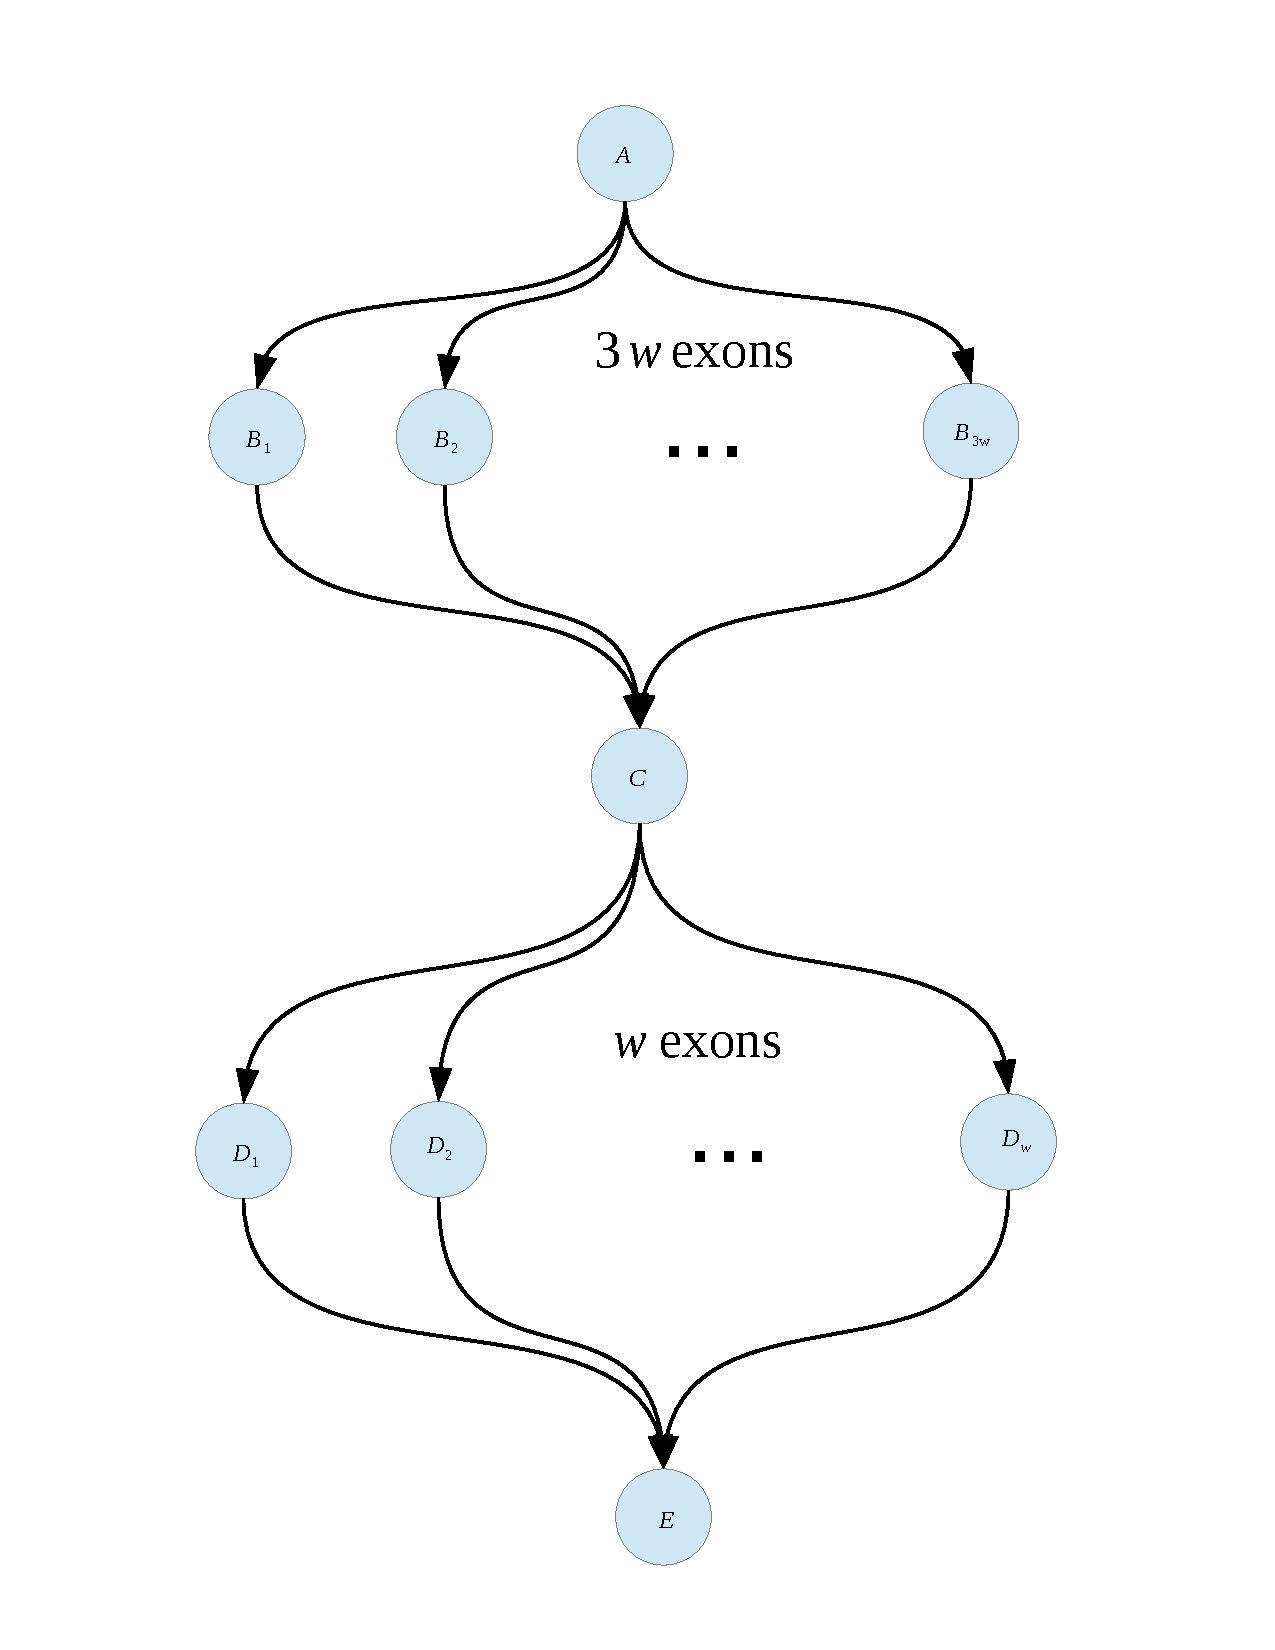
\includegraphics[width=1.0\textwidth]{figures/nphard/part3-gene.pdf}
\caption[一个 3-PARTITION 实例对应的 M-ISOFORM 实例的构造的基因]
{一个 3-PARTITION 实例对应的 M-ISOFORM 实例的构造的基因: 
这里每一个外显子的长度均为 $k-1$ bp ($k\geq 2$ 是一个固定的常数)。}
\label{tripart-reduce-gene}
\end{figure}

对于外显子 $A$, 在其中的 $k-1$ 个位置中的每一个位置共有 $wY$ 个读段将该位置作为起始位置, 
其中对于 $1\leq i\leq 3w$, 
这 $wY$ 个读段中有 $u(i)$ 个读段是从外显子 $A$ 连接到到外显子 $B_i$ 的。 

对于 $1\leq i\leq 3w$, 
外显子 $B_i$ 的 $k-1$ 个位置的每个位置均有 $u(i)$ 个读段将该位置作为起始位置, 
连接到外显子 $C$ 中。 

对于外显子 $C$, 其中的 $k-1$ 个位置的每个位置均有 $wY$ 个读段将该位置作为起始位置, 
其中对于 $1\leq i \leq w$,
这 $wY$ 个读段中有 $Y$ 个读段是从外显子 $C$ 连接到外显子 $D_i$ 的。 

对于 $1\leq i \leq w$,
外显子 $D_i$ 的 $k-1$ 个位置的每个位置均有 $Y$ 个读段将该位置作为起始位置, 
连接到外显子 $E$ 中。 

注意到, 由于所有的外显子的长度均为 $k-1$ bp, 而读段的长度为 $k$ bp, 
所以 $D$ 的所有位置中都没有是任何读段的起始位置。 

同时, 我们对于该 3-PARTITION 实例, 
对于图 \ref{tripart-reduce-gene} 中的所有的读段起始位置, 采样率均为 $1$。 

在此我们有了对应该 3-PARTITION 的实例的一个 M-ISOFORM 实例, 并且我们有一个如下的问题: 
\begin{center}
\fbox{\parbox{0.8\textwidth}{
是否存在一个剪切异构体的集合 $I$, $|I| \leq 3w$, 
以及这些转录本的表达量 $\lambda_i \geq 0$, $i \in I$, 
使得式 \eqref{rna-seq-data-poisson-likelihood} 中的似然函数
\begin{align}
\label{tripart-misof-likelihood-threshold}
L(R) &= \prod_{p\in P} \frac{{\lambda_p}^{N(p)} e^{-\lambda_p}}{N(p)!} \nonumber \\
&\geq \prod_{p\in P} \frac{{N(p)}^{N(p)} e^{-N(p)}}{N(p)!}
\end{align}
(这里所使用的阈值是 $\prod_{p\in P} \frac{{N(p)}^{N(p)} e^{-N(p)}}{N(p)!}$。)
}}
\end{center}

注意到, 前面对于给定的 3-PARTITION 实例构造这一个 M-ISOFORM 实例是在多项式时间之内完成的。 
下面我们说明给出的 3-PARTITION 有解当且仅当我们构造的着一个 M-ISOFORM 实例是有解的。 

首先我们容易看出来, 
对于下面的函数
\[
f(x) = \begin{cases}
0 & x < 0 \\
x^N e^{-x} & x \geq 0
\end{cases}
\]
其中 $N \in \mathbb{Z}^+$。 
该函数取得最大值当且仅当 $x=N$。 

所以, 式 \eqref{tripart-misof-likelihood-threshold} 成立当且仅当
\begin{equation}
\label{tripart-misof-equiv-lambda}
\lambda_p=N(p)
\end{equation}
对所有的 $p\in P$ 成立。  

我们首先说明在这里的 3-PARTITION 的实例有解时, 
我们所构造的 M-ISOFORM 的实例也有解。 
当该 3-PARTITION 的实例有解时, 假设 $i\in X$ 所属于的集合是 $X_j$, 
则我们给剪切异构体的集合 $I$ 中添加剪切异构体 
\[
A\to B_i \to C \to D_j \to E
\] 
同时将该剪切异构体的表达量定为 
\[
u(i)
\] 
此时 $I$ 中恰好有 $3w$ 个剪切异构体, 
并且根据式 \eqref{rna-seq-data-position-lambda} 我们知道式 
\eqref{tripart-misof-equiv-lambda} 此时也是满足的。 
另外这里容易看出来对于每个读段 $r\in R$, 
均存在一个剪切异构体 $i\in I$ 让读段 $r$ 是可以来自剪切异构体 $i$ 的。
所以我们知道对应的我们构造的 M-ISOFORM 实例也有解。 

下面我们说明当我们所构造的 M-ISOFORM 的实例有解时, 
这里的 3-PARTITION 问题也是有解的。 
我们容易注意到, 若存在满足要求的剪切异构体的集合 $I$ 时, 
其中一定包含恰好 $3w$ 个剪切异构体, 
因为图 \ref{tripart-reduce-gene} 所示的基因结构意味着至少有 $3w$ 个剪切异构体, 
这样才能保证对于每个读段 $r\in R$ 至少存在一个剪切异构体 $i\in I$ 
让读段 $r$ 是可以来自剪切异构体 $i$ 的。 
同时根据图 \ref{tripart-reduce-gene} 所示的基因结构, 
我们可以知道每个剪切异构体必须是
\[
A\to B_i \to C \to D_j \to E
\]
对于某 $1\leq i \leq 3w$ 和 $1 \leq j \leq w$, 
否则为了保证保证对于每个读段 $r\in R$ 至少存在一个剪切异构体 $i\in I$ 
让读段 $r$ 是可以来自剪切异构体 $i$ 的, 
我们需要 $I$ 中有多于 $3w$ 个剪切异构体。 
再注意到, 此时由于还有式 \eqref{rna-seq-data-position-lambda} 
和式 \eqref{tripart-misof-equiv-lambda} 的约束, 
对于前面的剪切异构体 $A\to B_i \to C \to D_j \to E$, 
它的表达量应该是
\[
u(i)
\]
同时, 根据式 \eqref{rna-seq-data-position-lambda} 
和式 \eqref{tripart-misof-equiv-lambda} 的约束, 
以及 $\frac{Y}{4} < u(x) < \frac{Y}{2}$, 
我们可以知道对于每个 $q\leq j\leq w$, 外显子 $D_j$ 中恰好有 3 个剪切异构体通过, 
并且这 3 个剪切异构体的表达量之和是 $Y$。 
所以在这个时候我们根据每个外显子 $D_j$, $1\leq j \leq w$ 中所经过的剪切异构体的情况, 
可以把 $X$ 分为不相交的 $w$ 个集合 $X_1$, $X_2$, \ldots, $X_w$ 使得 
对所有的 $1 \leq i \leq w$, $\sum_{x \in X_i} u(x) = Y$, 
并且每个 $X_j$, $1\leq j \leq w$ 中恰好有 $X$ 中的 3 个元素。 

所以该定理得证, 我们知道 M-ISOFORM 是一个 NP 完全问题。 

\end{proof}


